\documentclass{emulateapj}

\usepackage[utf8]{inputenc}
\usepackage{epsfig, floatflt}
\usepackage{graphicx}
\usepackage{float}
\usepackage{silence}
\usepackage{amsmath}
\usepackage{amsfonts}
\usepackage{amsthm}
\usepackage{amssymb}
\usepackage{listings}
\usepackage{color}
\usepackage[colorlinks]{hyperref}
\usepackage{textcomp}

\definecolor{url}{rgb}{0.1, 0.1, 0.4}

\lstset{inputpath = /home/torstein/Dokumenter/UiO/Fys3150/Fys3150_Project3/build-Scripts-Desktop_Qt_5_13_0_GCC_64bit-Debug}
\graphicspath{{/home/torstein/Dokumenter/UiO/Fys3150/Fys3150_Project3/build-Scripts-Desktop_Qt_5_13_0_GCC_64bit-Debug/}}
\hypersetup{colorlinks, urlcolor=url}


% Hvordan includere code snips
%\lstinputlisting{Filnavn! type kodefil}
%To crope lines shown insert
%firstline = <linenumber>, lastline = <linenumber>
%as kwarg

% Hvordan includere bilder
%\includegraphics[width=\linewith]{Filnavn! type png}
%To crop a picture insert 
%trim = {<left> <lower> <right> <upper>}, clip
%as kwargs



\begin{document}
	
	\title{Numerical integration}
	
	\author{Torstein Solheim Ølberg and Ada Mathea S. Veddegjerde}
	
	\email{torsteol@student.matnat.uio.no \\ amveddeg@student.matnat.uio.no \\}
	
	\altaffiltext{1}{Institute of Physics at the University of Oslo}
	
	\begin{abstract}
		We study the quantum mechanical expectation value of the correlation energy between two electrons which repel each other. We find this by calculating an integral using different integration methods. The methods we use are Gaussian Quadrature with Legendre and Laguerre polynomials, and Monte Carlo. We find that the Legendre polymonials do not give good enough results, and Laguerre, even though it gives better results, does not give very excact result and need to many summations. We had problems with using the Monte Carlo method. We expected it to give the most excact results, but it ended up giving us very wrong ones. Leading us to belive we may have done something wrong during our calculations.
	\end{abstract}
	
	\section{Introduction}
	\label{sec:introduction}
	In this paper we will be studying the wave functions of electrons, we will modell them like the single-particle wave function of an electron in the hydrogen atom. \par
	We want to find the quantum mechanical expectation value of the correlation energy between two electrons which repel each other via the classical Coulomb interaction, we get this by computing the integral \ref{eq:1}.\par
	We will attempt to compute the integral, and try different methods to achieve favorable results. The methods we will use are Gaussian Quadrature with both Legendre and Laguerre polynomials, and Monte Carlo methods.\par
	In the report we will start by going through all the theory we will use during our calculations. The we will go through what we did in the metods section. Our results will then be presented in graphs and tables in the results section. These results are what we later discuss and draw our conclutions from.
	
	\section{Theory}
	\label{sec:theory}
	\subsection{Particle Wavefunction} \label{sub:wave}
	The single-particle wave function for an election $i$ in the $1s$ state is given in terms of a dimentionless variable (the wave funcion is not properly normalized)
	$$
	\textbf{r}_i = x_i\textbf{e}_x + y_i\textbf{e}_y + z_i\textbf{e}_z,
	$$
	as
	$$
	\phi_{1s}(\textbf{r}_i) = e^{-\alpha r_i},
	$$
	where $\alpha$ is a parameter which we will fix equal to 2, corresponding to the charge of the helium atom $Z = 2$, and
	$$
	r_i = \sqrt{x_i^2 + y_i^2 + z_i^2}.
	$$
	
	The ansatz for the wave function for two electrons is then given by the product of two so-called $1s$ wave functions as $$
	\Psi (\textbf{r}_1,\textbf{r}_2) = e^{-\alpha (r_1 + r_2)}.
	$$
	The expectation value is given by:
	\begin{equation} \label{eq:1}
	\langle \frac{1}{|\textbf{r}_1 - \textbf{r}_2|} \rangle = \int_{-\infty}^{\infty} d\textbf{r}_1 d\textbf{r}_2 e^{2\alpha(r_1+r_2)}\frac{1}{|\textbf{r}_1 - \textbf{r}_2|}.
	\end{equation}
	Ignore the missing normalization factor.
	
	\subsection{Gaussian Quadrature} \label{sub:Gauss}
	The Gaussian Quadrature is a numerical integration method based on approximating an integral by a sum of a weight and a function at spesific points.
	\begin{equation*}
	I = \int_{a}^{b} f(x) dx \approx \sum_{i = 0}^{N} w_{i} f(x_i)
	\end{equation*}
	The weights are determined from a type of polynomial of order N and $x_i$ is the zero-points of that polynomial.
	
	\subsection{Weight Functions} \label{sub:weight}
	A weight function is defined to give the most exact results for a given polynomial. With it we get integration points defined spesifically for the shape of the polynomial it belongs to.
	
	\subsection{Legendre Polynomials} \label{sec:leg}
	Legendre polynomials are polynomials that solve the differencial equations
	\begin{equation*}
	C (1 - x^2) P + (1 - x^2) \frac{d}{dx} \left( (1 - x^2) \frac{dP}{dx} \right) = 0
	\end{equation*}
	For the Gauss-Legendre Quadrature the weights are then given by $2 L^{-1}_{0, i}$ where $L_{N, i}$ is the Legendre polynom of N-th order. The $i$ is a counter for the $x$ values, which are the null-points of the polynomial.
	
	\subsection{Laguerre polynomials} \label{sub:lag} 
	Laguerre polynomials are solutions of Laguerre's equation:
	$$
	xy''+(\alpha+1-x)y'+ny=0
	$$
	Note that this gives the generalized Laguerre polynomials, since $\alpha$ can have other values than zero. \\ \\
	The weight function for Laguerre polynomials is given by 
	\begin{equation} \label{eq:2}
	W(x)=x^{\alpha}e^{-x}
	\end{equation}
	This weight function is used to rewrite integrals, like so:
	\begin{equation} \label{eq:3}
	I=\int_a^b f(x) dx = \int_a^b W(x) g(x) dx \approx \sum_{i=0}^N w_i g(x_i)
	\end{equation}
	
	\subsection{Spherical coordinates} \label{sub:spher}
	One can switch to spherical coordinates like so:
	$$
	d\textbf{r}_1 d\textbf{r}_2 = r_1^2dr_1r_2^2dr_2d\cos(\theta_1)d\cos(\theta_2)d\phi_1d\phi_2,
	$$
	with
	$$
	\frac{1}{r_{12}}=\frac{1}{\sqrt{r_1^2+r_2^2-2r_1r_2\cos(\beta)}}
	$$
	and
	$$
	\cos(\beta)=\cos{\theta_1}\cos(\theta_2)+\sin(\theta_1)\sin{\theta_2}\cos(\phi_1-\phi_2)
	$$
	
	\subsection{Cosinus and Sinus Relation} \label{sub:cossin}
	It can be usefull to know that
	$$
	d\cos(\theta) = -\sin(\theta).
	$$
	And therefore
	$$
	\int_0^{\pi}d\cos(\theta) = -\int_0^{\pi}\sin(\theta)d\theta,
	$$
	\subsection{Monte Carlo Method}
	The Monte Carlo method selects N random numbers ($x_i$) in a given interval and use the numbers to evaluate the function $f(x_i)$. Summing the contributions we get gives us the final mean value 
	\begin{equation}
	\langle f \rangle = \frac{1}{N}\sum_{i=1}^N f(x_i) p(x_i),
	\end{equation}{}
	and standard deviation
	\begin{equation} \label{eq:undis}
	\sigma^2_f = \left( \frac{1}{N}\sum_{i=1}^{N} f(x_i)^2 - \left( \frac{1}{N}\sum_{i=1}^N f(x_i)\right)^2 \right) p(x_i)
	\end{equation}{}
	In the brute force method, with uniform distribution, $p(x_i)=1$.
	\section{Method}
	\label{sec:method}
	First we used the Gaussian Legendre Quadrature method to compute the integral \ref{eq:1} in C++ for N equal to 3, 4 and 5. We used the function gauleg from the lib.cpp library in \cite{1} to generate the . For some reason it was not possible to use $N = 6$ for this method, as the program either crashed or run for ever. Then we plotted the result for $N = 5$. \\
	
	Now we want to try improving our results. Therefore we will try using Laguerre polynomials \ref{sub:lag}.
	First we will switch \ref{eq:1} to spherical coordinates (\ref{sub:spher})
	\begin{align*}
	\int_0^{\infty} r_1^2dr_1 \int_0^{\infty}r_2^2dr_2 \int_0^{\pi}d\cos(\theta_1) \int_0^{\pi}d\cos(\theta_2) \\ \int_0^{2\pi}d\phi_1 \int_0^{2\pi}d\phi_2 \frac{e^{-2\alpha(r_1+r_2)}}{\sqrt{r_1^2+r_2^2-2r_1r_2\cos(\beta)}}
	\end{align*}
	We also see that we can use \ref{sub:cossin}, and insert this. (Note that the negative sign disappears). \\
	When we compute this we want to implement the function we integrate without the weight function \ref{eq:2}. With the way it is written now it is hard to exctract this weight function so we perform a change of variables. We define the new variables to be $u_1 = 2\alpha r_1$ and $u_2 = 2\alpha r_2$. \\
	Now we can easily exctract the weight function (\ref{eq:2}), which now looks like $u_1^2u_2^2e^{-(u_1+u_2)}$. We are left with
	\begin{align*}
	\frac{1}{(2\alpha)^5}\int_0^{\infty} du_1 \int_0^{\infty}du_2 \int_0^{\pi}d\theta_1 \int_0^{\pi}d\theta_2 \\ \int_0^{2\pi}d\phi_1 \int_0^{2\pi}d\phi_2 \frac{\sin(\theta_1)\times \sin(\theta_2)}{\sqrt{u_1^2+u_2^2-2u_1u_2\cos(\beta)}}
	\end{align*} \\
	
	Last, we implemented the Monte Carlo integration method, using the random number generator $std::uniform\_int\_distribution$ and N points ranging from one to 10 000.
	
	\section{Results}
	\label{sec:results}
	
	\begin{figure}
		\centering
		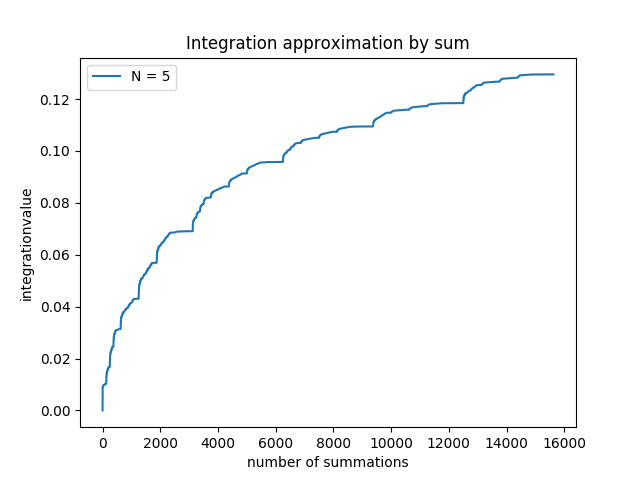
\includegraphics[scale=0.6]{Figur00.png}
		\caption{The integration sum by time. From using Legendre. A plot of the integration value as a function of the number of summations ($N^6$). The graph increases from zero in a pretty even curve, starting to flatten at about summation $6000$, but still rising at the last summation.}
		\label{fig:legint}
	\end{figure}
	
	\begin{deluxetable}{lc}
		\tablewidth{200pt}
		\tablecaption{Obtained values from Gaussian Legendre \label{tab:GLegQ}}
		\tablecomments{We see that that the value from the integration converges to something with higher values of N}
		\tablecolumns{2}
		\tablehead{N  & Values}
		\startdata
		3 & 1.05764 \\
		4 & 0.287955 \\
		5 & 0.129483
		\enddata
	\end{deluxetable}
	
	\begin{figure}
		\centering
		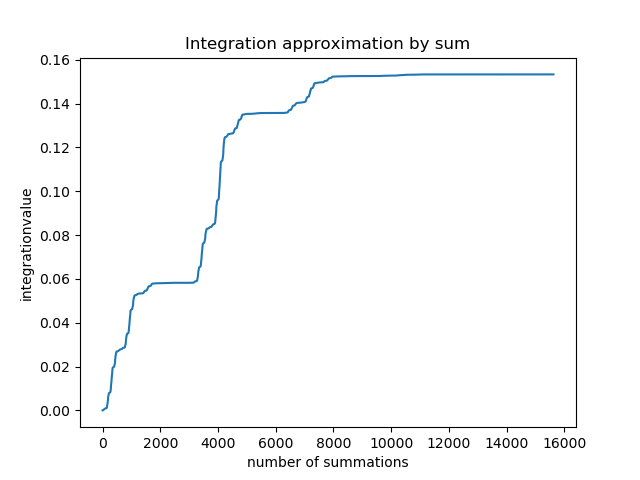
\includegraphics[scale=0.6]{Figure_1.png}
		\caption{The integration sum by time. From using Laguerre. A plot of the integration value as a function of the number of summations ($N^6$). The graph increases from zero untill it flattens at 0.15.}
		\label{fig:lagint}
	\end{figure}
	
	
	\begin{deluxetable}{lc}
		\tablewidth{200pt}
		\tablecaption{Obtained values from Gaussian Laguerre \label{tab:GLagQ}}
		\tablecomments{We see that that the value from the integration converges to something with higher values of N}
		\tablecolumns{2}
		\tablehead{N  & Values}
		\startdata
		3 & 0.118045 \\
		5 & 0.153304 \\
		10 & 0.178245 \\
		15 & 0.185254
		\enddata
	\end{deluxetable}
	
	\begin{figure}
		\centering
		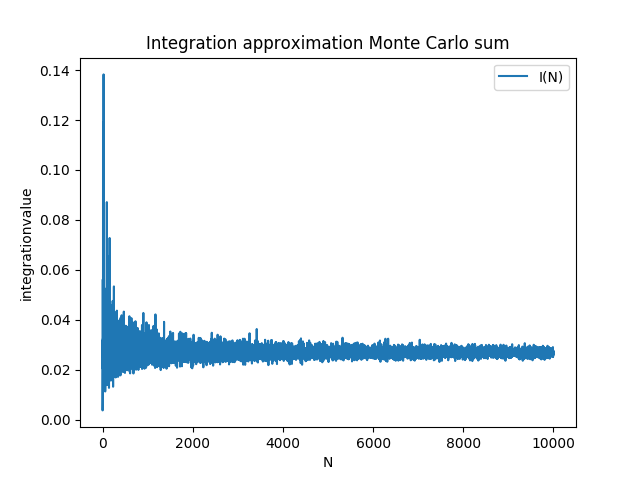
\includegraphics[scale=0.6]{Figur01.png}
		\caption{The integration value for increasing N for a brute force Monte Carlo integration. We see that it converges to some value around $0.03$ for larger and larger N.}
		\label{fig:BFMC}
	\end{figure}
	
	Figure \ref{fig:legint} is the integration value in our first attempt at calculating the integral. We tried calculating with different values of N, these result have been put in the table \ref{tab:GLegQ}. Figure \ref{fig:lagint} is the integration value after we changed to the Laguerre method. Here we tried with more N values, the result can be found in the table \ref{tab:GLagQ}. Figure \ref{fig:BFMC} shows the result of our brute force Monte Carlo integration for increasing values of integration points $N$. It is clear the it converges to som value around 0.03.
	
	\section{Discussion}
	\label{sec:discussion}
	The result we get from using the Legendre method is shown in \ref{fig:legint} and \ref{tab:GLegQ}. The integration is not very satisfactory, since the value we want to get is $\frac{5\pi^2}{16^2}\approx 0.1927657$ and the value we get is around 0.13 (\ref{fig:legint}). If we look at the table (\ref{tab:GLegQ}) we start at $1.06$ and get smaller values for bigger $N$, so the desired value is actually skipped between $N=4$ and $N=5$. Therefore this method is not particularly stable when $N$ is a low number. We assume the value will stabilize with higher values of $N$, but we are not able to test this as it requires too many calculations. \par
	
	Now we try the Laguerre method with the hope that we will get more accurate results. We show the results in the same format as we did the Legendre method, with \ref{fig:lagint} and \ref{tab:GLagQ}. Now we achieve better results. We still do not get a very accurate integration value, but now we can see that the graph (\ref{fig:lagint}) flattens out after about $8000$ summations, which tells us the integration value it has found is quite stable. the value varies quite alot for different values for N. Even with $N=15$, which is absurdly high for this method since it does too many summations to be effective, we do not get a very exact integration value. However in this method the integration value starts quite low and increases with higher $N$, therefore we can se that is  converges towards the correct integration value. \par
	
	The Monte Carlo method converges to a value around 0.03, which is way of the expected value. This might be because the implementation of the random number generator is faulty, giving an uneven distribution instead of a uniform distribution. The reason we believe there to be something wrong with the Monte Carlo Method is that we know from earlier that this type of integration method is good for multidimentional integrals.
	
	\section{Conclusions}
	\label{sec:conclusions}
	
	From the results we can see that the with larger N-th order polynomials for both Legendre and Laguerre Gauss-Quadrature gives better results, but they are not very satisfactory for the low level Ns we are able to use. However, we can see that the Laguerre method gives better results than the Legendre method in this case. Thus we can only conclude that in this specific case it is best to use Laguerre polynomials, thou we suspect the Monte Carlo method should actually performe better.
	
	
	% Hvordan lage en figur
	%\begin{figure}[t]
	%\includegraphics[width=\linewidth]{<filnavn>.png}
	%\caption{Description of figure -- explain all elements, but do not draw conclusions here.}
	%\label{fig:figure_label}
	%\end{figure}
	
	
	% Hvordan lage en tabell
	%\begin{deluxetable}{lccc}
	%\tablewidth{0pt}
	%\tablecaption{\label{tab:results}}
	%\tablecomments{Summary of main results.}
	%\tablecolumns{4}
	%\tablehead{Column 1  & Column 2 & Column 3 & Column 4}
	%\startdata
	%Item 1 & Item 2 & Item 3 & Item 4
	%\enddata
	%\end{deluxetable}
	
	
	
	\begin{acknowledgements}
		We want to thank God, Jesus and the all mighty Cuthulu for helping us on this article
	\end{acknowledgements}
	
	\begin{thebibliography}{}
		
		\bibitem[Ølberg og Veddegjerdet(2019)]{1} \ Project 3: \ Ølberg, Torstein Solheim; Veddegjerdet, Ada Mathea; 2019, \url{https://github.com/MrTorstein/Fys3150_Project3}
		
		%Hvordan sette oppe en referanse
		%\bibitem[Navnesen! et al.(år!)]{navnesen!:aar!} Tittel!.\ Navnesen!, N!, N!;
		%	Komisen!, K!., Vennesen!, V!. V!., osv.\ aar, Format!, side?!, linje?!, Utgiver!
		
	\end{thebibliography}
	
\end{document}